\documentclass[12pt]{article}

\usepackage{lmodern}
\usepackage[T1]{fontenc}
\usepackage[utf8]{inputenc}
\usepackage[spanish, activeacute]{babel}
\usepackage{listings}
\usepackage{enumitem}
\usepackage{graphicx}
\usepackage{float}
\usepackage[hidelinks]{hyperref}
\usepackage{xcolor}

\definecolor{mygreen}{rgb}{0,0.6,0}
\definecolor{mygray}{rgb}{0.8,0.8,0.8}
\definecolor{mymauve}{rgb}{0.58,0,0.82}
\lstset{
backgroundcolor=\color{mygray},
basicstyle=\ttfamily,
breakatwhitespace=false,
captionpos=b,
commentstyle=\color{mygreen},
deletekeywords={...},
escapeinside={\%*}{*)},
extendedchars=true,
keepspaces=true,
keywordstyle=\color{blue},
language=Octave,
morekeywords={*,...},
numbers=left,
numbersep=5pt,
numberstyle=\tiny\color{black},
showspaces=false,
showstringspaces=false,
showtabs=false,
stepnumber=1,
stringstyle=\color{mymauve},
tabsize=2,
}

\graphicspath {{ assets/images/ }}

\title{Prueba 2 - Api Restful}
\author{
    Wilson Aguilar \\
    \textsc{Plataformas Web}
}

\begin{document}

\maketitle

\section{Enlace a GitHub}

\url{https://github.com/WilsonAG/tech-impresoras}

\section{Enlace a Heroku}

\url{https://tech-impresoras.herokuapp.com/}

\section{Documentacion Postman}

\begin{figure}[H]
  \centering
  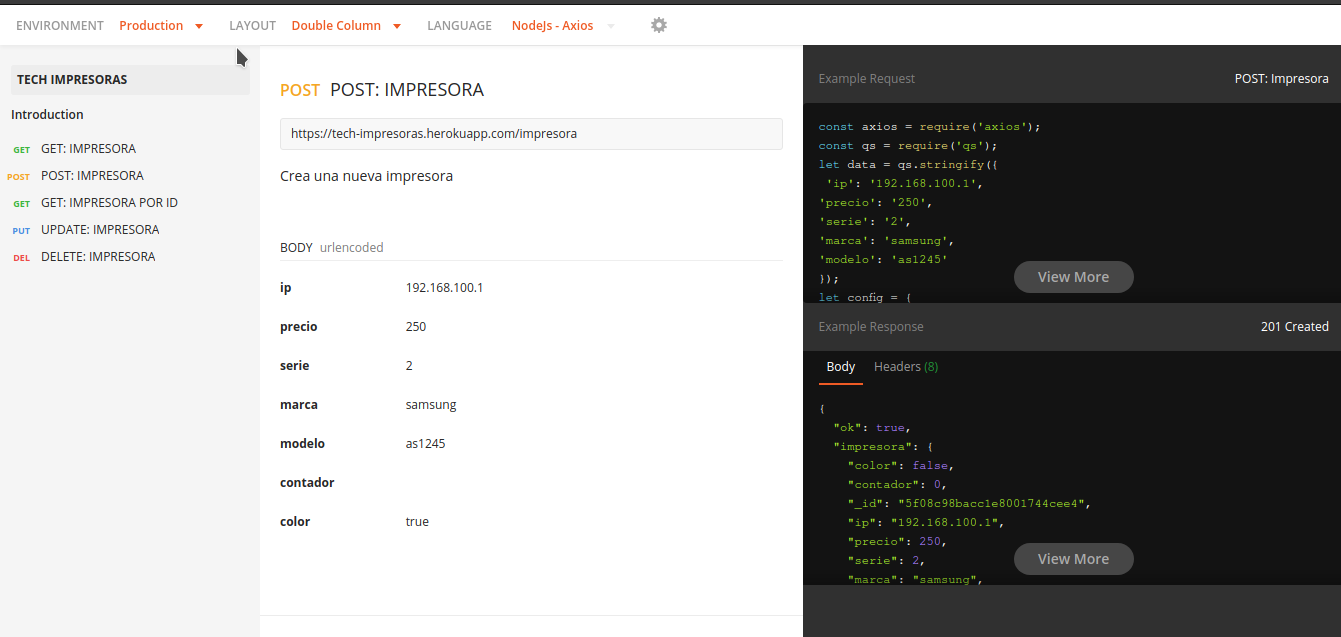
\includegraphics[scale=.3]{assets/images/postman.png}
  \caption{Documentacion}

\end{figure}

\url{https://documenter.getpostman.com/view/9801358/T17M7RDk}

\end{document}